\documentclass[border=2pt]{standalone}
\usepackage{tikz}
\usetikzlibrary{arrows.meta, positioning, decorations.pathreplacing}

\begin{document}
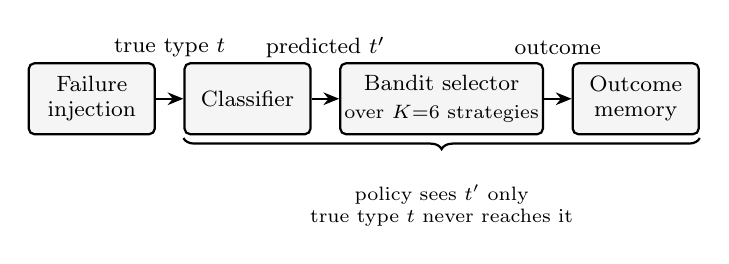
\begin{tikzpicture}[
  node distance = 3.5mm and 3.5mm,
  box/.style = {
    draw=black, thick, rounded corners=2pt,
    fill=black!4,
    minimum height=9mm, minimum width=16mm,
    align=center, font=\fontsize{8}{9}\selectfont, text=black,
    inner sep=1.5pt
  },
  arr/.style = {-{Stealth[length=2mm, width=1.6mm]}, thick, black},
  lbl/.style = {font=\fontsize{8}{9}\selectfont, align=center},
]

\node[box] (inj)  {Failure\\injection};
\node[box, right=of inj]  (clf)  {Classifier};
\node[box, right=of clf]  (sel)  {Bandit selector\\[1pt]{\fontsize{7}{8}\selectfont over $K{=}6$ strategies}};
\node[box, right=of sel]  (mem)  {Outcome\\memory};

\draw[arr] (inj) -- (clf) node[midway, yshift=6.5mm, lbl] {true type $t$};
\draw[arr] (clf) -- (sel) node[midway, yshift=6.5mm, lbl] {predicted $t'$};
\draw[arr] (sel) -- (mem) node[midway, yshift=6.5mm, lbl] {outcome};

\draw[decorate, decoration={brace, amplitude=4pt, mirror, raise=1pt}, thick, black]
     (clf.south west) -- (mem.south east)
     coordinate[pos=0.5] (bracemid);

\node[below=5mm of bracemid, font=\fontsize{7}{8}\selectfont, align=center, text width=48mm] (bracelabel)
     {policy sees $t'$ only\\true type $t$ never reaches it};

\end{tikzpicture}
\end{document}
